\documentclass[11pt]{report}            % Report class in 11 points
\usepackage{graphicx}		% Images
\usepackage[utf8]{inputenc}
\usepackage[T1]{fontenc}

%Math symbols
\usepackage{amsmath}		
\usepackage{amsfonts}
\usepackage{amssymb}
\usepackage{bm}
\usepackage{appendix}
%\usepackage{cleveref}

%Change margins
\usepackage[margin=1in]{geometry}

% Define toprule, midrule, bottomrule
\usepackage{booktabs}

%Font colors
\usepackage{xcolor}
\usepackage{color}

% Creating figures, flowcharts
\usepackage{tikz}
\usetikzlibrary{shapes.geometric, arrows,fit}


%Hyperlinks
\usepackage{hyperref}

\newcommand{\horrule}[1]{\rule{\linewidth}{#1}}
\newcommand{\tab}{\hspace*{3em}}


% Tikz definitions for flow charts
\tikzstyle{startstop} = [rectangle, rounded corners, minimum width=3cm, minimum height=1cm,text centered, text width=3.2cm, draw=black, fill=red!30]
\tikzstyle{io} = [trapezium, trapezium left angle=70, trapezium right angle=110, minimum width=1cm, minimum height=1cm, text width=2.2cm, text centered, draw=black, fill=blue!30]
\tikzstyle{ioq} = [trapezium, trapezium left angle=70, trapezium right angle=110, minimum width=1cm, minimum height=1cm, text width=2.2cm, text centered, draw=black, fill=white!30]
\tikzstyle{process} = [rectangle, minimum width=3cm, minimum height=1cm, text centered, text width=3.2cm, draw=black, fill=orange!30]
\tikzstyle{processq} = [rectangle, minimum width=3cm, minimum height=1cm, text centered, text width=3.2cm, draw=black, fill=white!30]
\tikzstyle{decision} = [diamond, aspect=2, minimum width=3cm, minimum height=1cm, text centered, text width=3.2cm, draw=black, fill=green!30]
\tikzstyle{arrow} = [thick,->,>=stealth]
\tikzstyle{line} = [ draw, -latex'] 

\parindent0pt  \parskip10pt             % make block paragraphs
\raggedright                            % do not right-justify

\title{\bf Battle of the Neighborhoods\\
For a brand new sports facility in Hyderabad, India}  % Supply information
\author{Sabarish Vadarevu}              %   for the title page.
\date{\today}                           %   Use current date.

\begin{document}                        % End of preamble, start of text.
\maketitle                              % Print title page.
\pagenumbering{roman}                   % roman page number for toc
\setcounter{page}{2}                    % make it start with "ii"
\tableofcontents                        % Print table of contents






\begin{abstract}
Highly populated cities like Hyderabad, India are in sore need of more sports facilities. Such facilities must be set up in suitable locations, lest they go unused and become too expensive to maintain. How do we find suitable locations? This question is answered in the present report. Venue data from Google Places API is used to find how locations of existing sports facilities are related to locations of other venues, such as restaurants, schools, gyms, etc... This relationship is then exploited to find other locations in the city that are most suitable for a new sports facility. 
\end{abstract}



\pagenumbering{arabic}                  % Start text with arabic 1


\chapter{Introduction}\label{chap:introduction}

{\color{purple} {\color{blue} Ajay} and {\color{black} Vijay} went to the same highschool over a decade ago. After going to different universities and working in different cities, they decide to catch up on some unremarkable day. They meet at a pub. Aged 30-something, they talk about how life has been, about career choices, and future plans. {\color{blue}Ajay} has worked for some finance firm or another, working with accounting, business planning, and so on... {\color{black} Vijay} has been jumping to and fro between IT roles and engineering jobs.

A few beers in...}

{\color{blue} Ajay: Life really hasn't been what I hoped it would be. I have decided to do something else. I have a decent bit of cash saved up to work on this new project.} 

Vijay: I told you already, dog-whisperer sounds fun, but it's not going to take off. 

{\color{blue} Ajay: Not that one, although I insist dog-whisperer is going to be a mainstream profession any day now. Enough about that. I'm talking about investing in sports.}

Vijay: You mean like those competitions where dogs jump through hoops and run through tunnels? 

{\color{blue} Ajay: No. Not that one either. Nothing about dogs. I'm serious. I want to invest in sports. I want to see more people playing more sports. Remember back when we used to play cricket on the streets? Or fought with other groups of kids for a spot on a ground?}

Vijay: Oh yeah. I remember that. I also remember that one time when you guys egged me on to confront that senior from school, but ran away like headless chickens when he started punching me. I ran up a fever after that and had to stay in bed for 2 days, and you guys ...

{\color{blue} Ajay: Let's not worry about what happened over ten years ago. My point is, the sports infrastructure in the city was shiet. It's worse now, because all of those empty spots we claimed for cricket are gone, used up for construction of some residence or business or something else. There's too many cars parked on the streets, so kids today can't even play on the streets like we used to.}

Vijay: They could play at school...

{\color{blue} Ajay: Really? At school? Did you forget where we went to school?}

Ahem... You must admit that playing cricket on the rooftop and running down three floors of stairs to bring back a ball had a certain appeal to it. 

{\color{blue} Yeah, right. My point is, most schools don't have playground. There are no decent parks. Even if there are, the parks are off limits for kids to play at. All of the vacant grounds are being used up. Streets have too much traffic and parked cars. There's really no place for kids to play at. And forget about adults. When was the last time you played something?}

Last week I think

{\color{blue} Computer games don't count!}

Alright. Fine. I see your point. There are very few sports facilities. I think I can see where you are going. You want to build a sports facility, right? It is going to be quite expensive. Just the cost of leasing the land will be very high, what with the real estate boom in the city? And installing a surface? Do we even have any of that in the city? Maintenance? Forget about it.The facility is going to be in tatters within a month. Look at brand new airports and railways in the country. A few months and they're garbage. And that is in spite of having armies of personnel to look after them. Can you afford any of that?

{\color{blue} Sigh... If there is a nice indoor volleyball court in the street next to yours, and you can play there everyday for the cost that's twice a gym membership, would you go play?}

Of course. But that's just wishful thinking. There aren't any volleyball courts like that. 

{\color{blue} There are. Quite a few of them actually. You can book a court for an hour for about a thousand rupees. Split that among 10 players, and that's a hundred bucks. Play 3 days a week, that costs you 1,200 rupees a month. How does that sound?}

No way! Why haven't I heard of this before. Where is this sports hall you're talking about. If there really is one nearby, I'd definitely go. 

{\color{blue} That's the problem. There aren't many of them. At least not for volleyball. There are a lot more indoor sports halls for badminton. They usually charge about INR 400 per hour per court. They are well maintained. Don't expect air-conditioned halls, but expect clean courts and reasonable ventilation. There are a few apps going around that help you book these courts or find players to team up with.}

Problem solved then, isn't it. So, do you want to invest in publicizing these facilities?

{\color{blue} No. There are far too few of these facilities. Nowhere near enough to cover all of the sports enthusiasts in the city. I want to build more of these facilities. Starting with just the one. Hopefully, over a few decades, I can expand to cover the entire city. We can have lots of coaching camps, seasonal tournaments, scholarships, live telecasting. We can make proper sports leagues out of all this. In a nation that is dominated by cricket, I believe we can make a real difference if we can build sports infrastructure at this grassroots level. We can then move to other cities in the state, maybe the country.}

Okay. Time out. Two things. First, you seem to know what you're talking about. I'm impressed, and that's not just the beer talking. Second, who is this "we"? While I'm happy to patronize your sports facilities, if you ever get them running, I'm far too poor to be investing on this scale. 

{\color{blue} I have a few other people interested. I haven't spent the past decade working with businesses for nothing. I've schmoozed my way through a lot of people interested in sports infrastructure. In fact, we are halfway through putting together a proposal to get some venture capital. We have the business plan and the initial capital. The issue we're working on right now is location. I'd love to set up our first facility close to where I live, but I don't know if that's a good idea. We've been arguing over this for a week now, and still couldn't agree on a location.}

Hmmm... Location indeed. That is an interesting question. In fact, let me google a few things. 

You're right. There are quite a few existing sports facilities. They're not all businesses though. Quite a few belong to colleges and governmental organizations. In any case, it shouldn't be hard to use these locations to train a model and extract a few candidate locations. 

{\color{blue} Train a model. Why are we getting into using models. Beautiful young ladies do have that charm that can help a business case, but that's really not something I'm keen on.}

<Facepalm> That is not what I mean. I'm not talking about models that show up in advertisements and fashion shows. I mean machine learning, artificial intelligence. Are you sure you have worked with businesses for the better part of ten years?

{\color{blue} Ah! Hahaha. I see. Don't look at me like I'm an idiot. There isn't much of that kind of modelling going on in the businesses I work with. I see your point. I'm not good at that stuff though. In fact, I know next to nothing, and neither do any of my partners.}

I kind of figured that when you thought of supermodels. I might be able to help. It just so happens that I have recently been dabbling in data science and machine learning. I'm looking for a pet project to build some proper experience. This could be just the thing I'm looking for. 

{\color{blue} Really? You can help me do this? That would really help me out. But are you sure you can do it, considering your inexperience. What if you get it wrong? I might lose a lot of money, you know.}

Whoa! Cool it. I'm offering to do it for no pay, and you're already ready to pile it on me? If that's how it's going to be, then I'm not doing it. You can find your own way to figure out the best location, and convince your partners and your investors for its suitability. 

{\color{blue} You know what? That just might do the trick. You will train this model thing. And we can then tweak it a little bit to get it to work for me. I can then show it to my investors. They won't argue with me when they see all of the fancy maths.}

Nope. Not a chance. I will help you, but I'll not do your dirty work. Tell you what. I'll do the modelling bit. I explain how all of it works. You can then take it, learn what you can, and tinker with it to see if it helps your case. 

{\color{blue} Hmmm... Okay. That sounds fair.}

I'm not done yet. Whenever we meet to talk about the work I'm doing for you, we'll meet at a fancy pub. And you foot the bill. Deal?

{\color{blue} Deal.}

\chapter{Methodology}\label{chap:methodology}


Vijay: Right. Let's get down to business before the booze gets to us. 

{\color{blue} Ajay: Good. What are we talking about?}

I will outline how we will approach this problem. The actual problem-solving will come later. But first, we must establish the expect outcomes for this little project. 

{\color{blue} Yes. We want to identify a location to build a sports facility.}

Almost. We will have to be more specific though. Here's how I will define it. 

\section{Problem statement}

\textbf{Problem statement:} Identify a set of locations that are most suitable to establish a new sports facility in Hyderabad. The suitability of a location is expressed as a suitability score that lies between 0 and 1, 0 indicating an unsuitable location, and 1 indicating a highly suitable location. To this end, we will train models that capture the relationship between the suitability score for a location and the distance to other points of interest in the vicinity. The trained model will later be used to find locations that maximize the suitability.

{\color{blue} I am a bit lost. Can we break this down into simpler parts? }

Okay. Let me draw this out in a flowchart. 

\section{Strategy}
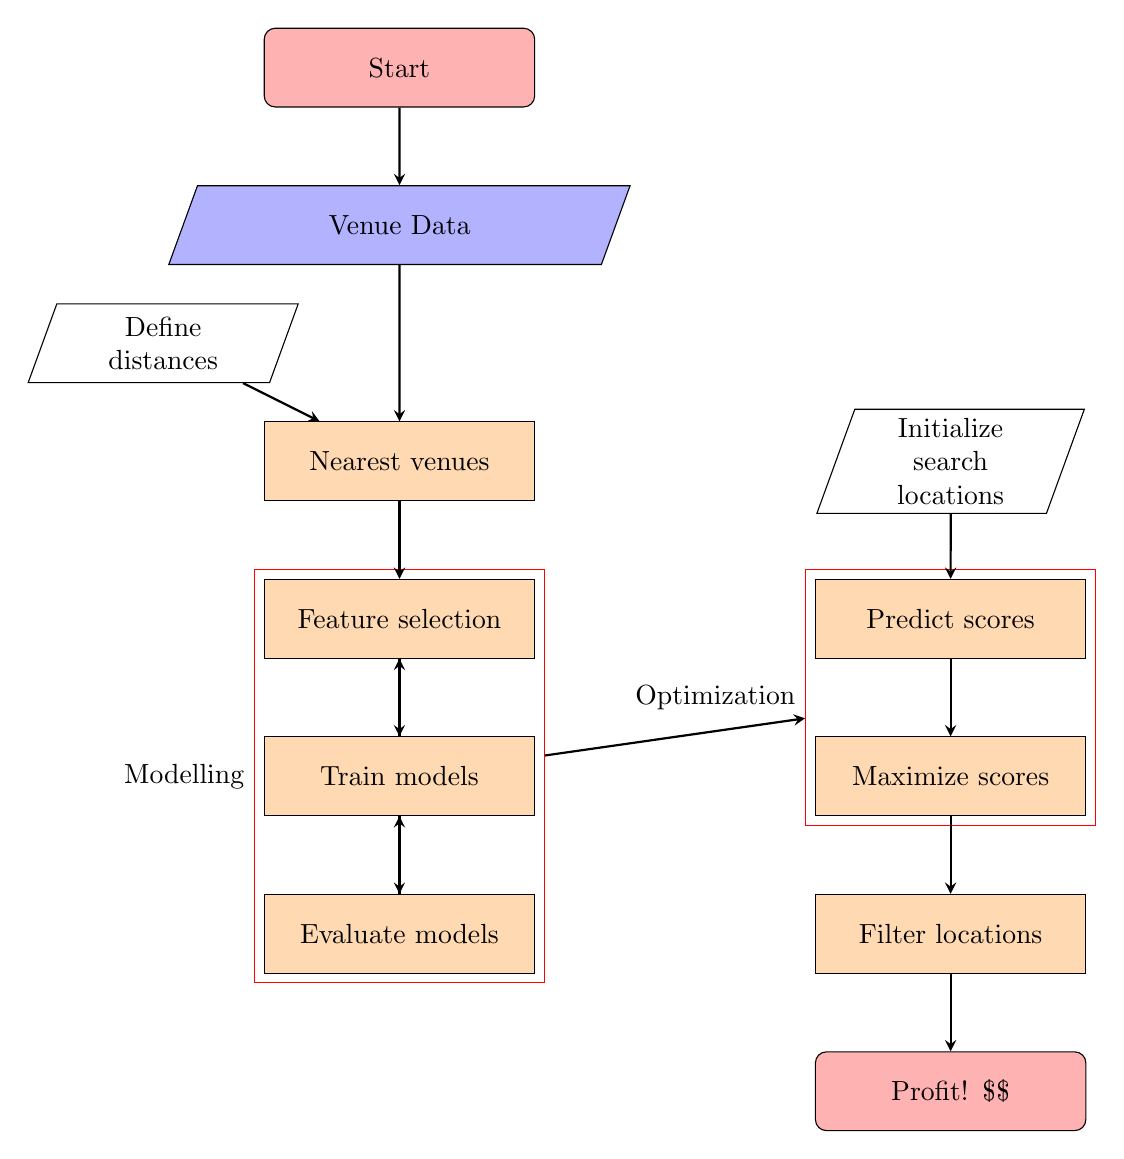
\begin{tikzpicture}[node distance = 3cm]
	\node (start) [startstop] {Start};
	\node (data) [io, below of=start, yshift=1cm] {Venue Data};
	\node (distance) [ioq, left of=data, yshift=-1.5cm] {Define distances};
	\node (preproc) [process, below of=data] {Nearest venues};
	\node (features) [process, below of=preproc, yshift=1cm] {Feature selection};
	\node (models) [process, below of=features, yshift=1cm] {Train models};
	\node (evaluate) [process, below of=models, yshift=1cm] {Evaluate models};
	\node[draw=red, fit=(features) (models) (evaluate)] (modelling) {};
	\node[left] at (modelling.west) {Modelling};

	\draw [arrow] (models) -- (evaluate);
	\draw [arrow] (evaluate) -- (models);
	\draw [arrow] (start) -- (data);
	\draw [arrow] (data) -- (preproc);
	\draw [arrow] (distance) -- (preproc);
	\draw [arrow] (preproc) -- (features);
	\draw [arrow] (features) -- (models);
	\draw [arrow] (models) -- (features);


	\node (init) [ioq, right of=preproc, xshift=4cm] {Initialize search locations};
	\node (predict) [process, below of=init, yshift=1cm] {Predict scores};
	\node (optimize) [process, below of=predict, yshift=1cm] {Maximize scores};
	\node (filter) [process, below of=optimize, yshift=1cm] {Filter locations};
	\node (stop) [startstop, below of=filter, yshift=1cm] {Profit! \$\$};
	\node[draw=red, fit=(predict) (optimize)] (optimizer) {};
	\node[left] at (optimizer.west) {Optimization};

	\draw [arrow] (modelling) -- (optimizer);
	\draw [arrow] (init) -- (predict);
	\draw [arrow] (predict) -- (optimize);
	\draw [arrow] (optimize) -- (filter);
	\draw [arrow] (filter) -- (stop);
\end{tikzpicture}


Let me run you through the flowchart. We first collect data on all kinds of venues from Google Places. You know Google Places, right? That's the system that gets Google Maps to work. We find locations of places like restaurants, gyms, banks, pubs, etc... 

{\color{blue} I'll stop you there for a bit. Why do we care about gyms and banks and pubs? What do their locations have to do with a sports facility?}

I'm glad you asked. The ideal location for your new sports facility should be one that has good access to transport, is in a place with a reasonable population density, and isn't too expensive to lease. Or perhaps not. We don't know. We must do two things. First, we must figure out what qualities we want in a neighborhood to build the sports facility. Second, we must find neighborhoods with these qualities. These ``qualities'' that I just mentioned, what could they be? I think that the distribution of venues such as supermarkets, pubs, restaurants, gyms, etc... are a good proxy for these qualities. 

{\color{blue} I see. So we look at other venues of interest to characterize neighborhoods. I guess the modelling part of it is to express this characterization in a mathematical model. Yes?}

Exactly. We don't know how to characterize neighborhoods. Is having lots of banks a good thin? What about colleges? Should there be lots of restaurants and no gyms? We'll let our model figure all of that out. 

{\color{blue} What's with the little ``Define distances"? And the boxes on the right?}

Ignore that ``Define distances" box. That's for the nerds. The chart on the left is for the first part I mentioned earlier -- figuring out what qualities we want in a neighborhood. We use data on existing sports facilities to work this out. Once we have all of that information built into a model, we go look for neighborhoods that maximize these qualities. That is what the chart on the right does. It takes the model we built, and work its way through lots of locations in the city. This optimization part spits out a bunch of locations that are most suitable for the sports facility. You can then take this to your partners and investors to sort out the specifics. 

{\color{blue} I understand. Kind of. Can we get into the details of the boxes?}


Next time. It's better to show than tell. In the meantime, have a look at \href{https://github.com/saba-vadarevu/IBM-dataScience-Capstone/blob/master/final/intro_data.ipynb}{this notebook} if you want more details on how it's done.

\chapter{Data Collection}\label{chap:data}


As I said earlier, we'll get our data from Google Places. They provide data on lots of venues for free, although there are some restrictions on it. If you want to know how you can get this data, have a look at \href{https://github.com/saba-vadarevu/IBM-dataScience-Capstone/blob/master/final/intro_data.ipynb}{this notebook}. It will explain how I pull data from Google Places. 

{\color{blue} So we are using banks, cinemas, colleges, gyms, hospitals, pubs, restaurants, schools, and supermarkets. Why these? What about auditoria or temples or police stations?}

Because, reasons. 

{\color{blue} What reasons?}

Reasons. 

{\color{blue} Which are...}

Reasons.

{\color{blue} Okay, I can see where this is going. Fine. All I care about is that this makes sense. Does it?}

We'll know at the end. Look, if you paid me to do this for you, I would spend a few weeks researching on how best to do this. You're not. So I'm not. We will know at the end if any of this makes sense. We are using nine different kinds of venues. That's something. 

{\color{blue} Fine.}


\section{Data Sample}
Here's what our data looks like. These are five existing sports facilities that are closest to the center of the city. 

\input{../sports}

{\color{blue} I see. Wait. What center of the city? I didn't know there was one.}

Well, I didn't either. So I took it upon myself to nominate a place to be the center of the city. This makes my analysis a lot easier. I used the Buddha statue in Hussain Sagar lake as the center. If you look at the geometry of the city, the centroid does fall roughly near this point, so it's all good.

{\color{blue} Wow. Okay. You're weird, you know that? I suppose the `Dist\_CC' column is for distance from this city center that you designated? }

Yep. In metres. 


{\color{blue} So, how did you get this data?}


\section{Google Places API}

Why, using Google of course. Not the way you're thinking of though. Google Places has an API which gives you different kinds of information when you submit different kinds of requests. Have a look at \href{https://github.com/saba-vadarevu/IBM-dataScience-Capstone/blob/master/final/intro_data.ipynb}{this notebook} for details on how to make these requests.

The requests that I have used are called `Nearby Search' requests. These requests work like this. I specify a keyword and a location. The API returns venue information matching the keyword near the specified location. There are two ways to make this request. I can either specify a radius about the specified location, or ask for all results in increasing order of distance from the specified location. The first option restricts results by distance, the second sorts them by distance. I used the second. 

{\color{blue} Because why?}

Because, reasons. Don't look at me like that, this time there are reasons for doing this. Venues like banks or restaurants aren't uniformly distributed in the city. Google Places only returns 20 results per request, up to a total of 60 results for the specified location and keyword. If I use the first kind of `Nearby Search' request, it's easy to miss a lot of venues wherever they are densely packed. Unless I use a very fine grid for the search. A finer search grid takes too long to. Using the second kind of result sidesteps this issue. Again, go have a look at \href{https://github.com/saba-vadarevu/IBM-dataScience-Capstone/blob/master/final/intro_data.ipynb}{this notebook} for details.

{\color{blue} You know what, I'll just leave it to you to worry about the details. We have information on lots of venues now. How many venues have we got? }

\section{Number of venues}
Let me put the numbers in a table. 

\begin{tabular}{ll}
\toprule
Venue Category & Number of results \\
\midrule
Banks 		& 2281 \\
Cinemas		& 287 \\
Colleges 	& 1718 \\
Gyms 		& 1325 \\
Hospitals 	& 374 \\
Pubs		& 664 \\
Restaurants	& 309 \\
Schools 	& 3993 \\
Sports 		& 730  \\
Supermarkets 	& 503 \\
\bottomrule
\end{tabular}

For illustration, I plotted the locations of all of the existing sports facilities on a map in fig. \ref{fig:existing-sports}. 

\begin{figure}
	\centering
	\includegraphics[width = 0.95\linewidth]{existSports.png}
	\caption{Locations of existing sports facilities in Hyderabad, from Google Places API\label{fig:existing-sports}}
\end{figure}

{\color{blue} That doesn't look right. Just 309 restaurants and 374 hospitals int he city? And 503 supermarkets? Surely there are many more.}

You are absolutely right. There are indeed a lot more supermarkets than 503. What I have done here is pick only a few chains of supermarkets -- More, Heritage Fresh, Reliance Fresh, Ratnadeep, and Big Bazaar. Because there are too many tiny supermarkets and just a lot of other stores labelled as supermarkets. Restricting our data to these few chains produces more consistency. After all, the presence or absence of a Heritage Fresh in the neighborhood does say something about the neighborhood. 

It is the same for restaurants. I picked a few chains and then looked for the locations of every restaurant belonging to the chain -- MacDonald's, Subway, KFC, Pizza Hut, Domino's Pizza, Burger King, Paradise Biryani, and Karachi Bakery. 

There is a different problem with hospitals. Apparently, a lot of the smaller clinics aren't tagged as hospitals in Google Places. Or they are tagged, but don't show up for some reason. Most of the hospitals returned by the API are the large multispeciality ones. Except in the outskirts in the city, where smaller clinics also show up.

There is some inconsistency in the data. Some entries in supermarkets and restaurants don't actually belong to the chains I wanted to capture. The hospitals aren't all of the same size and scale. There are also a lot of non-sports-related venues in the data for sports facilities. Or sports retail stores. Overall, however, the relevant entries outnumber the irrelevant ones; so we're good to go.

{\color{blue} I may be wrong here, but aren't you supposed to clean your data before using it to make predictions? I'm no data scientist, and even I know that.}

Yep. I should. I will have to manually comb through the data and discard inappropriate entries. That is a boring and time-consuming process. If you were paying me to do this, I would have done that. For a pet project with no pay, this will have to do. As I said before, the number of appropriate datapoints is far greater than the number of inappropriate ones. 

There's one other limitation, one I've already mentioned. A lot of places aren't indexed by Google Places. And some of the indexed places could be missing from the data because of the limitations on the number of results returned by the API. These are things that we'll just have to live with.  

{\color{blue} Is there nothing we can do to fix these issues?}

We could go look for data from other cities in India that could be similar to Hyderabad. It's not a lot of extra work, but it will increase the size of our datasets, and consequently the runtime. I may have a go at it at a later time, but not for now. 


\chapter{Preprocessing}\label{chap:preprocessing}

{\color{blue} Are we ready to train the models then? }

Not quite. Remember what we wanted to do with our models? We want to characterize neighborhoods using data on different venues located within and around the neighborhood. To do that, we need a way to pick out the venues that are close to any particular location. 

{\color{blue} Is that hard to do?}

Not at all. This is a common problem used in machine learning called `Nearest Neighbors Search'. There are a lot of software libraries that I can directly use to get this done, so we don't have to worry about how to implement it. Have a look at \href{https://github.com/saba-vadarevu/IBM-dataScience-Capstone/blob/master/final/preprocessing.ipynb}{this notebook} to see how I implement nearest neighbors search to find venues close to a specified location. 

{\color{blue} Okay. Looks easy enough. So we are choosing 10 nearest neighbors. Why 10?}

Because 10 is a nice number. Ten is actually an upperlimit. We will later try and see if we can get away with fewer venues when characterizing a neighborhood.

{\color{blue} Fine. What is this about defining distances.}

We use latitude and longitude to identify the location of any point in the city. We need a function to give us distances between two points given their latitudes and longitudes. There are, again, libraries that can do this for us. We need to keep the time taken to compute these distances to a minimum though, because we'll have to compute distances for a LOT of pairs of points. So, we define our own function that calculates approximate distances, but really fast. 

{\color{blue} That makes sense. Are we ready to do the training then? }

Relax man. We'll get there. If we want to train a model, we need datapoints. In our case, the datapoints will be lots of locations in the city, and the distances to nearest venues of different categories. Later, we will use these distances to create what we call `features' and `labels' that we use to train models. 

We have a way to obtain distances to ten nearest venues of each venue category for any specified location. Now, we just have to pick out a whole bunch of locations that we want to use as datapoints. Obviously, we should use the locations of existing sports facilities. We want our models to know that the locations of existing sports facilities are suitable locations for sports facilities. If they weren't, these facilities would probably have been used for some other purpose. In addition to existing sports facilities, we will choose points randomly in the city. Again, the details are all in \href{https://github.com/saba-vadarevu/IBM-dataScience-Capstone/blob/master/final/preprocessing.ipynb}{this notebook}. The number of random points we'll use is ten times the number of existing sports facilities. Because, reasons.

We have a lot of locations in the city. We have a method to obtain distances to ten nearest venues for each of this locations. We use this method. That produces a large dataset containing 8,030 locations and associated distances. We'll save a copy of this dataset on disk for later use. 

{\color{blue} Since you've stopped, I'm assuming we are now ready to start training our models?}

Indeed we are.

\chapter{Modelling}


\subsection{Targets}
{\color{blue} Alright! Let's get training.}

After just one little thing. There are two ways to do machine learning. Supervised and unsupervised. We will do supervised learning first. That means, we give the model a target to aim at. In unsupervised training, there isn't any target to aim at; we just want the model to group together different datapoints that look similar. 

{\color{blue} What target do we want our model to be aiming at?}

That is an important question. We want the target to reflect the suitability of a location for setting up a sports facility. Let's call this a ``suitability score''. We will have this suitablity score be between 0 and 1. If the suitability score is 0, then the location is unsuitable. If the suitability score is 1, then the location is highly suitable. 

{\color{blue} Okay. What exactly is this suitability score?}

That remains to be defined. I came up with this simple definition:
\begin{equation}
	\begin{aligned}
		p_n(\text{sports}) &= \frac{1}{1+\frac{d_n(\text{sports})}{0.5}}, \\
		S &= p_0(\text{sports}),
	\end{aligned}
\end{equation}
where $d_n(\text{sports})$ is the distance to the $n^{th}$ closest sports venue, $p_n(\text{sports})$ is the `proximity' to the $n^{th}$ closest sports venue defined above, and $S$ is the suitability score. The suitability score is based on proximity to just to closest sports venue. Note that the subscript $n$ is zero-based, so a subscript zero means first closest venue. 

For any location that coincides with the location of an existing sports facility, the suitability score is 1. 

{\color{blue} I think I understand what's going on. Proximity is defined so that it always takes values between 0 and 1. Why do you have the factor $0.5$ though?}

That acts to scale the distances. Basically, it makes proximity go to $0.5$ when the distance to the $n^{th}$ nearest venue is 0.5km. With regards to the suitability score, this means the score drops to 0.5 when we move to a location 0.5km away from an existing sports facility. It just feels nicer to have a scaling that makes sense to me. You are free to use a different scaling if you want. 

{\color{blue} Would the results of the modelling change if we use different scaling factors?}

Yes, they would. 

{\color{blue} And let me guess. You don't want to try different scaling factors because I'm not paying you to do this.}

Yep. 


\subsection{Features}
{\color{blue} We have a target to aim at. From what I understand, we also need some input to go into the model, yes?}


Yes, we do. These inputs are called features. Usually, a lot of work goes into deciding what features to use. In fact, that is the reason we collected distances to 10 nearest venues for 9 different venue categories. We are hoping that all of these distances can provide a meaningful set of features that can adequately characterize neighborhoods. Should we use all of the 10 distances, or just a few? Or should we use `proximity' defined above? After all, proximite goes from 0 to 1, which is a nice property to have. 

{\color{blue} Why are you asking me? I am absolutely clueless about what to use.}

Unfortunately, so am I. We will try them all out. Specifically, I have defined four different functions, dist\_n, dist\_0\_n, prox\_n, and prox\_0\_n. These functions use the 9 sets of 10 distances for each location and spit out a vector. See \href{https://github.com/saba-vadarevu/IBM-dataScience-Capstone/blob/master/final/model_binary.ipynb}{this notebook} for details.  
We will try to use feature vectors produced by each of these four functions and see which one gives us the best accuracy. 


\section{Binary classification}

{\color{blue} The notebook is called `model\_binary'. What's with the binary?}

The binary refers to binary classification. In this kind of modelling, we say that our data belongs to two classes -- suitable locations, and unsuitable locations. We have to assign these labels when training our data. 

{\color{blue} Let me guess. Locations with suitability scores less than 0.5 are unsuitable, and those with suitability scores greater than 0.5 are suitable?}

Yep. To be precise, those with suitability score greater than \textbf{or equal to} 0.5 are suitable. There is this library called Scikit-learn that has models ready to go. I will spare you the details of getting these models to run. Suffice it to say that I tried all four feature functions for different `n', where `n' is the rank of the venue in terms of distance from the location. Some feature functions did better than others, but the overall performance wasn't so good.

{\color{blue} Really?! I was getting excited about this. It sounded like it should really work.}

Well, our problem just doesn't happen to suit binary classification. Remember how we collected a lot of random locations in the city to build a dataset? Most of these locations fall far from existing sports facilities, and are consequently labelled as unsuitable. There are a lot more of these locations than suitable locations. This imbalance makes it quite messy to have a reasonable accuracy with the model. 

{\color{blue} Can't we just drop those extra points?}

We can, but then the dataset we have will be very biased in terms of what neighborhoods it represents. We can't take a model trained on this dataset and expect it to make predictions on random locations in the city. 

{\color{blue} How about adding more datapoints near existing sports facilities?}

We could do that. But then all of the models we train will have a large error associated with them, and it becomes hard to compare models. 

{\color{blue} So there's no way to fix this?}

I'm not sure. To be honest, I just don't want to do this binary classification. Ultimately, we want don't want just any suitable location, we want the most suitable location. That is, we want our locations to be ranked in terms of suitability scores. If we are aiming for a continuous target to facilitate ranking, then using binary classification isn't the best idea. 

{\color{blue} Didn't you have some probabilities associated with the predictions?}

Yes, there are probabilities associated with the predictions. And you are right, we can find the locations with the greatest probability. It just feels a bit too artificial though, to assign discrete labels, and then rank them on probability. We might as well skip this step and just work with continuous targets all the way. 

{\color{blue} Alright. What's the next step then?}


\section{Linear Regression}

%\chapter{Conclusion}\label{chap:conclusion}

{\color{blue} What am I missing then?}

Any machine learning model is only as good as the data that goes into it. We tried a few different things in terms of features, but we didn't pay a lot of attention to the targets -- the suitability score. 

{\color{blue} It makes sense to use a suitability score that goes from 0 to 1. What's wrong with that?}

The problem is with the way we assigned suitability scores to datapoints. We used proximity to nearest sports venue. I argued that if a sports facility exists at a location, it means that the location is suitable. That's not the strongest argument. 

Sports facilities associated with governmental organizations usually have little to do with profitability. There are also a lot of isolated tennis courts and such that are in our dataset. Land allocation is sticky. Businesses can go bankrupt and give way to others, but sports facilities in governmental organizations, schools, parks, etc... are not subject to the profitability or suitability of the sports facility itself. Rather, they depend on the success of the larger facility that they are part of. 

We assigned low suitability scores to locations that are far from existing sports facilities. Do you see the contradiction here?

{\color{blue} Hmmm.. I think I do. There are no suitable locations in the city, except for those that are already occupied by sports facilities. So the model is designed to fail from thestart.}

Not completely. There is bound to be a lot of noise in any data. Existing sports facilities are not ideally distributed. And some locations that are suitable for a sports facility are currently unoccupied. We hope that when we supply sufficient data to a reasonably simple model, then all of this noise is smoothened out. In the predictions of the model, some of the existing sports facilities will have a suitability score less than 1, and some locations that are sufficiently far from existing facilities will have a score very close to 1. 


{\color{blue} We hope that would happen, but it is not guaranteed.}

Indeed. But that is the best we can do for now. So, go ahead and pitch this to your investors, but remember the shortcomings of the whole thing. 

{\color{blue} Will do. Cheers!}

%\input{conclusion}
%\input{references}

\begin{appendices}
\input{app_VenueData}
\end{appendices}

\end{document}
